%\begin{figure}[ht]
%    \centering
%    \includegraphics[width=0.5\textwidth]{3_modeling/figures/algoFigure6.pdf}
%    \caption{Elementary substrate block 3D schematic.}
%    \label{fig:algo}
%\end{figure}
%
%\begin{figure}[ht]
%    \begin{Verbatim}[frame=single]
%        .subckt elementary_bloc D F L R Re U
%        R1 U N001 RH
%        R2 N001 D RH
%        R3 Re N001 RL
%        R4 N001 F RL
%        R5 N001 L RL
%        R6 R N001 RL
%        .ends elementary_bloc
%    \end{Verbatim}
%    \caption{Elementary substrate SPICE netlist}
%    \label{fig:subSpiceNetlist}
%\end{figure}

\begin{figure}[ht]
    \centering
    \begin{subfigure}{0.32\textwidth}
        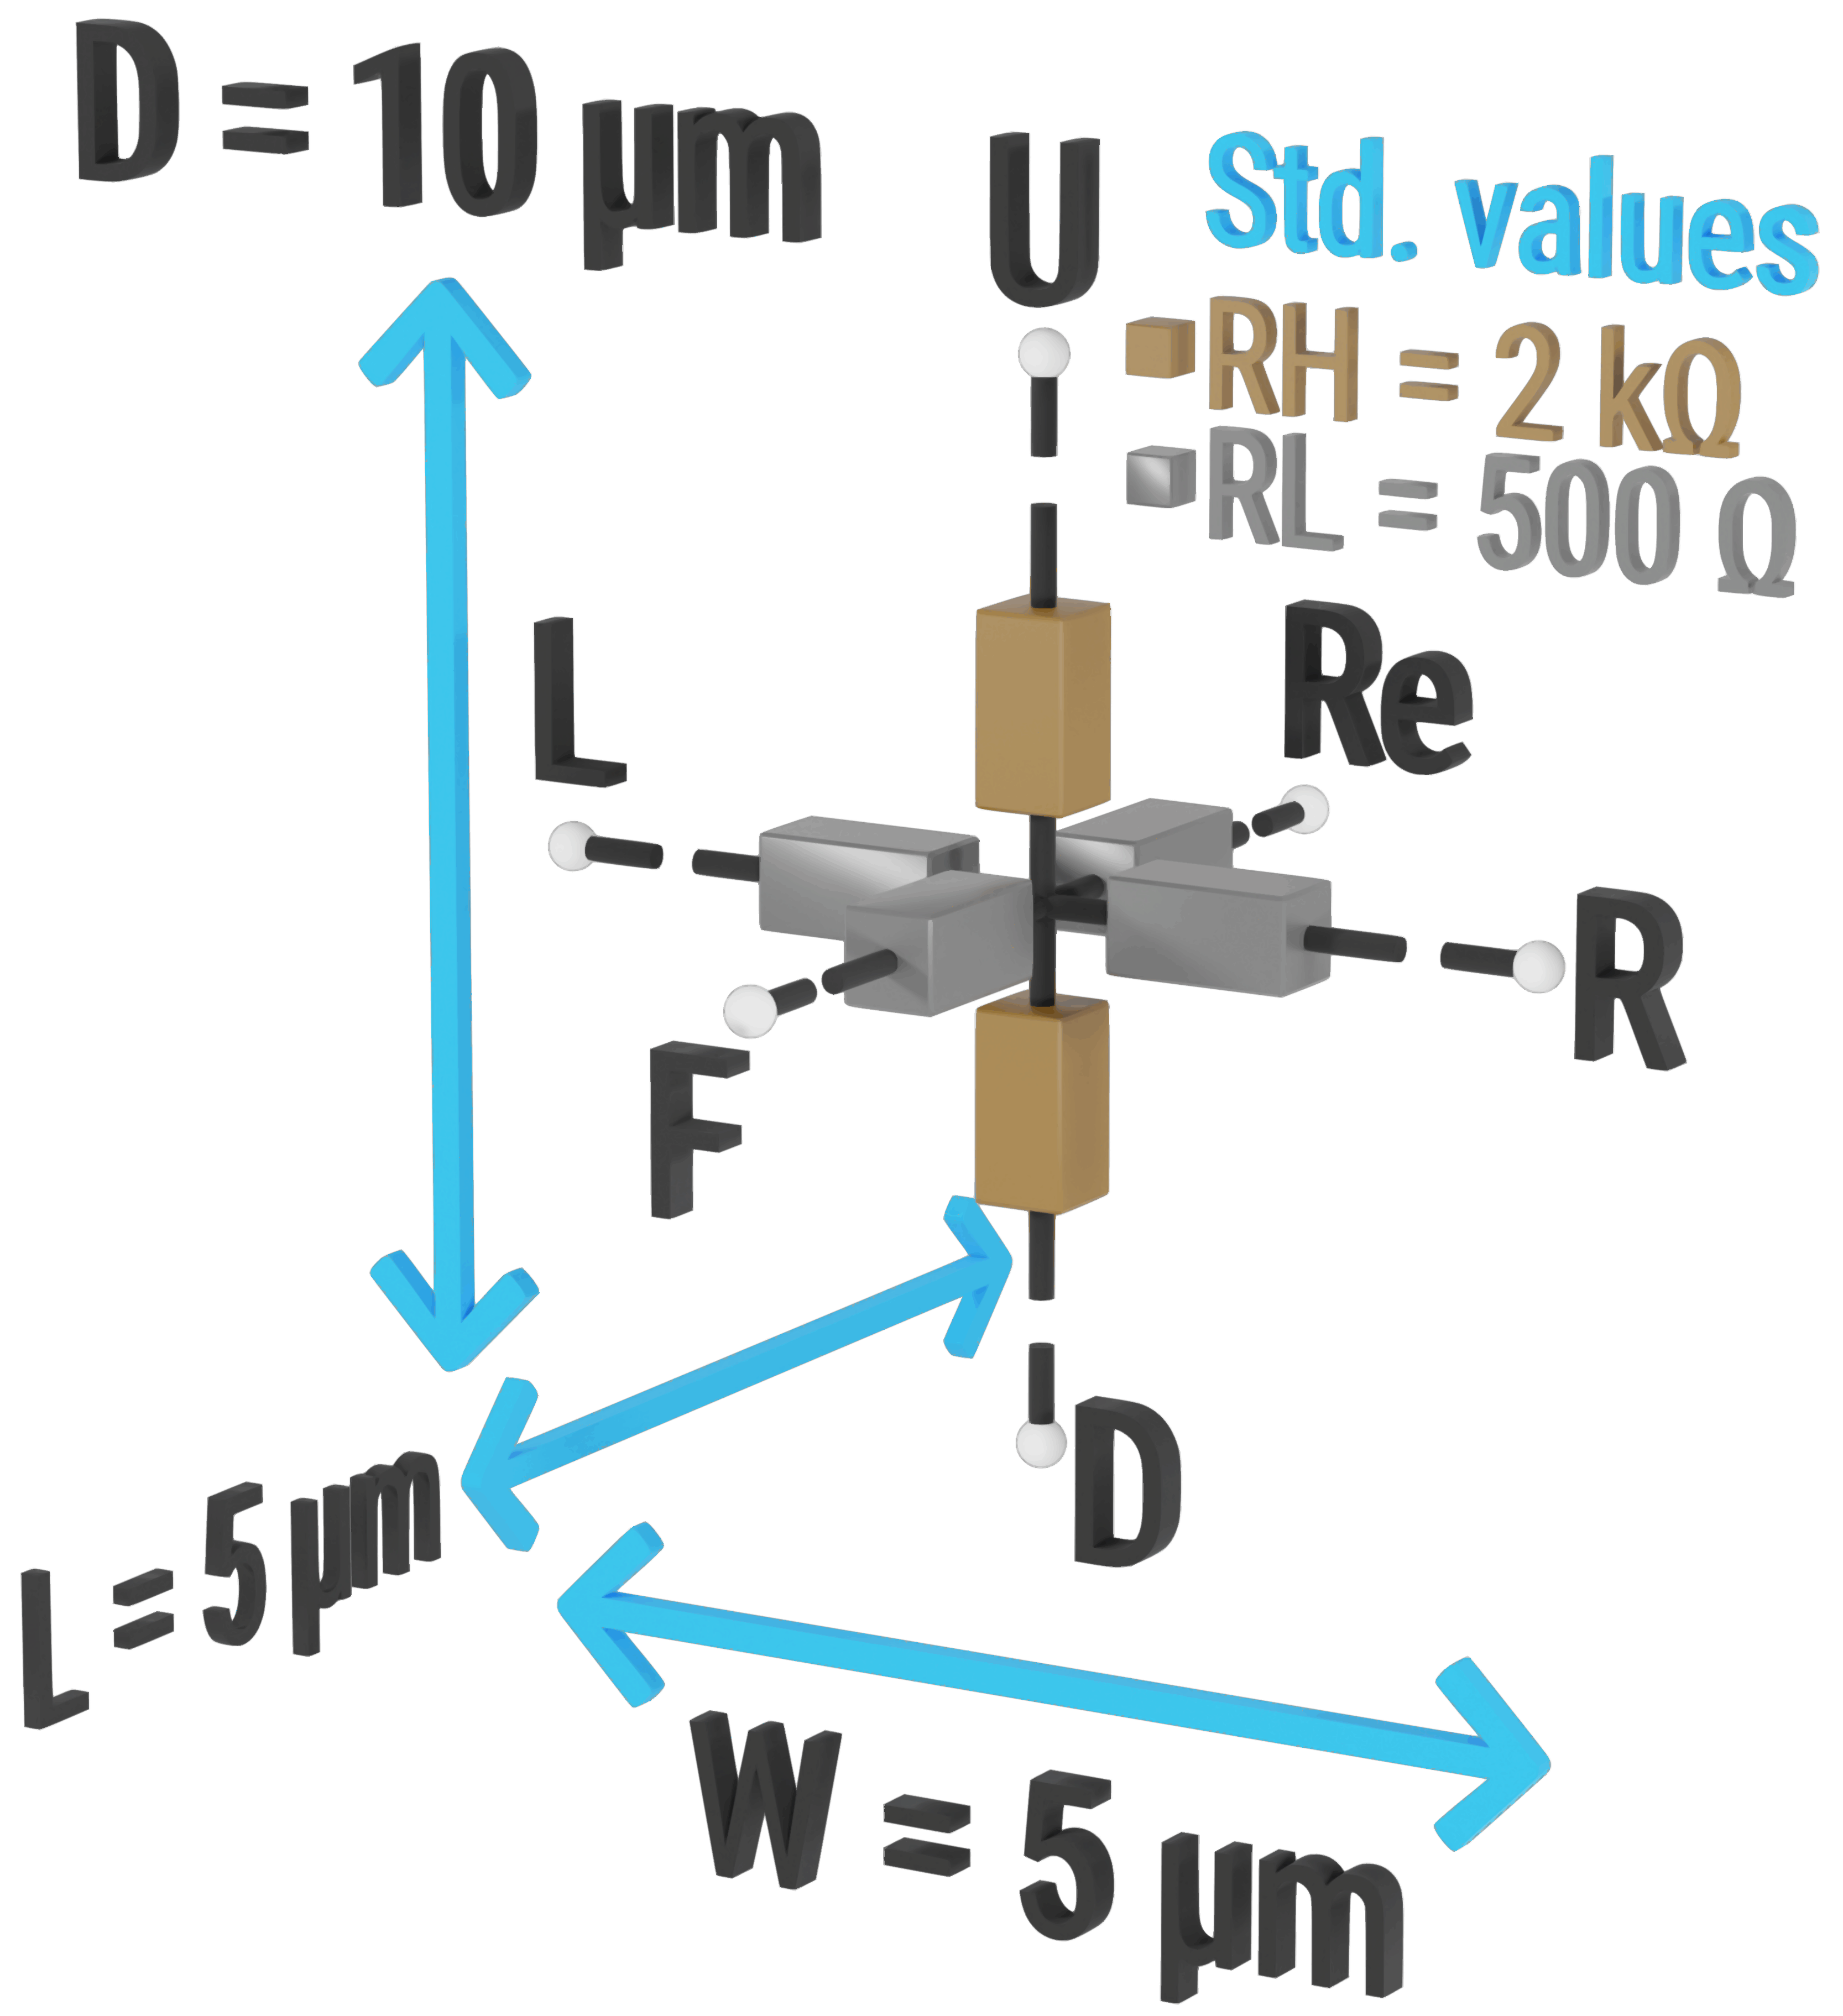
\includegraphics[width=\textwidth]{3_modeling/figures/algoFigure8.pdf}
        \caption{Elementary substrate block 3D schematic with the default values used for our technology and the SPICE in-out names.}
        \label{sfig_elemSub}
    \end{subfigure}
    \hfill
    \begin{subfigure}{0.60\textwidth}
        \begin{Verbatim}[frame=single]
.subckt elementary_bloc D F L R Re U
R1 U N001 RH
R2 N001 D RH
R3 Re N001 RL
R4 N001 F RL
R5 N001 L RL
R6 R N001 RL
.ends elementary_bloc
        \end{Verbatim}
        \caption{Elementary 6-resistors substrate SPICE netlist description, with the in-out names in accordance with Fig. \ref{sfig_elemSub}.}
        \label{sfig_spiceNetSub}
    \end{subfigure}
    \caption{Elementary substrate building block 3D schematic and its SPICE netlist.}
    \label{fig:elemSubAndNetlist}
\end{figure}
